\chapter{Semantics}\label{chap:semantics}
Semantics is the meaning of a language and the pragmatic of it. It covers the internal behavior of the running programs, when referring to computer science.

The semantics are defined in different ways. The most common ways are denotational, operational and axiomatic semantics. This report uses the operational semantics to define how the semantics works for the language \lang{}.
\section{Type Rules}\label{sec:TypeRules}
The language \lang{} has the types \{num, text, bool\}. They contain the variables that can be seen in figure \ref{fig:InTypeRules}.

\begin{figure}[H]
\noindent\makebox[\linewidth]{\rule{\textwidth}{0.4pt}}
    \textbf{\lang{}: Beginner Friendly Game language} \\
    \textbf{Type}
    \begin{enumerate}  
        \item float 
        \item string
        \item boolean
    \end{enumerate}
    \textbf{KeyWords}
    \begin{enumerate}  
        \item num : float 
        \item text : string 
        \item bool : boolean 
        \item Vector : float, float
    \end{enumerate}
    \textbf{Variables}\\
    Variables can be any combination of the upper and lower case letters from a to z and numbers from 0 to 9, provided that the first character is not a number.\\
    \noindent\makebox[\linewidth]{\rule{\textwidth}{0.4pt}}
    \caption{Informal Type Rules}
    \label{fig:InTypeRules}
\end{figure}

A type environment is a partial function \[E : \textbf{Var} \cup \textbf{Pnames} \rightharpoonup \textbf{Types}\]
The environment is updated with 
\[ \textbf{E}[x\mapsto T] \] 
and the type environment \textbf{E'} defined by
\[\textbf{E'(y)} = \bigg \{ \quad \begin{aligned}  E(y) \\ T \end{aligned} \quad \begin{aligned} if\ y \neq x \\ if\ y = x \end{aligned}\quad \bigg \} \]

\lang{} is able to add a num with a num arithmetically and a text with a text using concatenation. Furthermore, it is able to add a text with num with concatenation by implicitly converting the num to a text.\\
\[ \textbf{[TextAdd]} \frac{E \vdash e_1 : type_1 \quad E \vdash e_2 : type_2}{E \vdash e_1 + e_2 : text}\quad \textbf{Where}\: \begin{aligned} type_1\: ,\ type_2\: \in \{text, num\} \\   type_1\ or\ type_2\ is\ text \end{aligned}\]
All the other arithmetical operators - subtraction, multiplication, division, modulus and unary - are not usable on text, as these only work on nums.
\[ \textbf{[Arithmetic]} \frac{E \vdash e_1 : num \quad E \vdash e_2 : num}{E \vdash e_1\ op\ e_2 : num}\quad \textbf{Where}\: op\: \in \{+,-,*,/\}\]
Furthermore, relational operators can be used on two nums creating a bool. These operators are: and, or, greater than, less than, greater than or equals, less than or equals, equals and not equals.

\[ \textbf{[Relational]} \frac{E \vdash e_1 : num \quad E \vdash e_2 : num}{E \vdash e_1\: op\: e_2 : bool}\quad \textbf{Where}\: op\: \in \{<,<=,>,>=,=,!=\}\]
\[ \textbf{[Gates]} \frac{E \vdash e_1 : bool \quad E \vdash e_2 : bool}{E \vdash e_1\: op\: e_2 : bool}\quad \textbf{Where}\: op\: \in \{and,or\}\]

Furthermore, unary can be used on a single num, creating a new num:
\[ \textbf{[Unary]} \frac{E\, \vdash e_1 : num }{E\, \vdash -e_1 : num}\]
The boolean expression 'not' takes a bool and returns a bool.
\[ \textbf{[Not]} \frac{E\, \vdash e_1 : bool }{E\, \vdash !e_1 : bool}\]

Some relational operators can also be used on two texts, namely equals and not equals, comparing whether a text is identical to the other: 
\[ \textbf{[Less]}\frac{E\, \vdash e_1 : text \quad E \vdash e_2 : text}{E\, \vdash e_1\ rel\ e_2 : bool}\quad \textbf{Where}\ rel \in \{=,!= \}\]

To check if the type of x is the same type that is declared, variables are defined as:
\[ \textbf{[Var]}E \vdash x : type\quad \textbf{if}\ E(x)  = type\]

A function is called by taking a number of expressions as parameters that each have a type, which can return a variable:
\[ \textbf{[Fcall]}\frac{E\, \vdash e_1:type_1\ ...\ E\, \vdash e_n:type_n}{E\vdash f(e_1,\ ...\ ,\ e_n):type}\quad \textbf{Where}\ E(f)=(type_1\: \, ...\: ,\ type_n)\rightarrow type\]

The function gets a list of parameters in the start - \(x_1\ ...\ x_n\) - and a type for each of them. It also has a return variable, whose type is defined under compile time:
\[\textbf{Func-Dcl]} \frac{\langle D_M\: ,\ E[f \mapsto (type_1\: ,\ ...\: ,\ type_n \rightarrow type)] \rangle \rightarrow E'}{\langle f(type_1\ x_1\: ,\ ...\: ,\ type_n\ x_n):type\ begin\ B\ end\ D_M\: ,\ E \rangle \rightarrow E'}\]
In the var declaration, variable x and its type get connected. Afterwards, the type environment gets updated with information:
\[ \textbf{[Var-Dcl]} \frac{\langle D_V,E[x \mapsto type ]\rangle \rightarrow E'}{\langle dcl\ type\ x\ D_V\: ,\ E \rangle E'}\]
\[\textbf{[Empty-Dcl]} \langle \varepsilon, E \rangle \rightarrow E \]

In Block, \(D_V\) and \(M_C\) are checked if they return void. In Prog 1 and 2, it is \(\{D_V\: ,\ S\}\) and \(\{D_C\: ,\ P\}\) respectively. This is done because they, by being void, are type correct. Everything has to have a type, and if these return a void, it means they have run correctly.
\[\textbf{[Block]} \frac{\langle D_V, E \rangle \rightarrow E' \quad E' \vdash M_C:void}{E \vdash \{D_V,M_C\}:void}\]
\[ \textbf{[Prog 1]} \frac{\langle D_V, E \rangle \rightarrow E' \quad E' \vdash S:void}{E \vdash \{D_V,S\} : void}\]
\[\textbf{[Prog 2]} \frac{\langle D_C, E \rangle \rightarrow E' \quad E' \vdash P:void}{E \vdash \{D_C, P\}:void}\]

In ForUp and ForDown, the x and e are checked if they are num. B is checked if it returns void.
\[\textbf{[ForUp]} \frac{E(x) = num \quad E \vdash e:num \quad E \vdash B:void}{E \vdash for\ x\ upto\ e\ do\ B\ end:void}\]
\[\textbf{[ForDown]} \frac{E(x) = num \quad E \vdash e:num \quad E \vdash B:void}{E \vdash for\ x\ downto\ e\ do\ B\ end:void}\]

In While, the boolean expression is checked if it is a bool. B is checked if it is void.
\[\textbf{[While]} \frac{E(b) = bool \quad E \vdash B:void}{E \vdash while\ b\ do\ B\ end:void}\]
\section{Abstract Syntax}
In this section, the abstract syntax for \lang{} is presented. The abstract syntax does, unlike the grammar for the parser, not take precedence into consideration, but rather gives a more readable understanding of what is possible in the language. It is written for human readers, as computers do not understand the various ambiguities that are present in the abstract syntax.
The syntactic Categories contains all the fundamental parts and some meta variables like b and a that stand for the Boolean Expression and the Arithmetic Expression respectively. The full abstract syntax is seen on figure \ref{fig:AS}.

\begin{figure}[H]
    \centering
    \begin{lstlisting}[escapeinside={(*}{*)}]
Syntactic Categories
(*
\(n \in \textbf{Numerals}\) \\
\(t \in \{true\: ,\ false\} \) \\
\(x \in \textbf{Primitive Variable}\) \\
\(y \in \textbf{Reference Variable}\) \\
\(b \in \textbf{Boolean Expression}\) \\
\(a \in \textbf{Arithmetic Expression}\) \\
\(S \in \textbf{Statement}\) \\
\(P \in \textbf{Program}\) \\
\(e \in \textbf{Expression} \) \\
\(D_V \in \textbf{Variable Declaration} \) \\
\(D_C \in \textbf{Class Declaration}\) \\
\(D_M \in \textbf{Method Declaration} \) \\
\(C_M \in \textbf{Method Call} \) \\
*)

Formation rules
(*
P ::= \(D_V\) \(M_C\) | \(D_C\) P \\
S ::=  set x to e | set y to new Class(\(e_1,\ ...,\ e_n\)) | skip | \(S_1\) \(S_2\) | 'if' b 'then' \(B_1\) 'else' \(B_2\) 'end' | 'for' x 'upto' e 'do' B 'end' | 'for' x 'downto' e 'do' B 'end' | 'while' b 'do' B 'end' | f(\(e_1,\)\ ...,\ \(e_n\)) \(C_M\) | return e | return y \\
a ::= n | \(a_1+a_2\) | \(a_1-a_2\) | \(a_1*a_2\) | \(\frac{a_1}{a_2}\) | \(a_1\: \%\: a_2\) | \((a_1)\) \\
b ::= \(a_1\) = \(a_2\) | a1 > a2 | a1 < a2 | a1 <= a2 | a1 >= a2 | a1 != a2 | b1 and b2 | b1 or b2 | not b1 | (b1) | t \\
B ::= \(D_V\) S \\
\(D_V\) ::= dcl type x \(D_V\) | dcl classname y \(D_V\) |  \(\varepsilon\) \\
\(D_M\) ::= dcl func x(\(type_1\ e_1,\ ...,\ type_n\ e_n\)) begin B end \(D_M\) | \(\varepsilon\) \\
\(D_C\) ::= class ClassName begin B \(D_M\) end\\
\(M_C\) ::= class main begin \(D_V\) S end
*)
    \end{lstlisting}
    \caption{The syntactic categories and formations rules of \lang{}}
    \label{fig:AS}
\end{figure}

In the formation rules, the different syntactic categories, and what they stand for, are described. In the two variable types - primitive and reference - the naming has to start with an uppercase letter, from A to Z, or lowercase letter, from a to z, optionally followed by a number of uppercase letters, lowercase letters and numerals, from \underline{0} to \underline{9}.
\subsection{Small step semantics and big step semantics}
Operational semantics can be defined with small step semantics and big step semantics. Big step semantics define a single transition from the starting point of \(\gamma{}\) to the end state of \(\gamma{}'\), whereas in the small step semantics the state \(\gamma'\). The transitions are shown with an arrow \(\rightarrow{}\!\!\) in big step semantics and a double lined right arrow \(\Rightarrow\) in small step semantics. Big step semantics are in most cases able to define the semantics, but when describing parallelism or non-determinism, big step semantics are not able to define the semantics correctly, whereas small step semantics can. Big step semantics are easier to formulate, making them the preferred choice when defining semantics in this report, since \lang{} does not contain non-determinism, ruling out the advantages of small step semantics.
\section{Operational semantics of \lang{}}
\label{sec:OpSemantics}
This chapter describes the operational semantics of \lang{}. To describe the name binding mechanism of \lang{}, the environment-store model described in the book \textit{Transistions and Trees} \cite{stoloc} is used.
In the environment-store model, variable environments are used to assign to each variable name a specific location, which can be interpreted as a memory address.
The value associated to a given location can be retrieved using a "store" function, which maps a location to its corresponding value. This name binding model can be seen on figure \ref{fig:Env}.
An environment function \(\mathbf{Env_V}\) is a partial map in \(\mathbf{Env_V}\), defined as follows, where 'next' is the reserved word for mapping to the next available location:
\[ \mathbf{Env_V} = \textbf{Var} \cup \{next\} \rightharpoonup \textbf{Loc} \]

where \(\mathbf{env_V}\) denotes an arbitrary member of \(\mathbf{Env_V}\). \\ \\
\[\mathbf{Env_C} = \textbf{Cnames} \rightharpoonup \textbf{Stm} \times \mathbf{Var^n} \times \mathbf{Env_V} \times \mathbf{Env_M}\]
A class environment needs a name to be able to distinguish itself from other class environments, since there can be more than one class environment. The class environment needs to hold the information about the variable and method inside of it, and there is used static scope rules on the class and method.
\[\mathbf{Env_M} = \textbf{Mnames} \rightharpoonup \textbf{Stm} \times \mathbf{Var^n} \times \mathbf{Env_V}\] 



In the following, it is assumed that the amount of locations is enumerable, which makes \(\mathbf{Loc} \simeq \mathbb{N} \), and \(new: \mathbf{Loc} \rightarrow \mathbf{Loc}\), where the newest used location returns  the next available locations that has never been used previously. It can be defined as \(new\ l = l+1\). \\
\textbf{Sto} is a set of partial maps defined as \(\textbf{Sto} = \textbf{Loc} \rightharpoonup \textbf{Val}\)
Where \textbf{Val} is the set of all possible values.

When a class is instantiated, a heap is needed to manage all the objects that are made, with all the variables for that instance of the class. \[\textbf{Heap} = \textbf{HeapNames} \mapsto \textbf{Loc} \] As shown, the heap is a collection of different locations where the information for the different classes are stored. A new store that can have those class is also needed. This store is defined as: \[\textbf{Sto} = \{next\} \mapsto \mathbf{Env_V} \times \textbf{Cnames} \]

\begin{figure}[H]
    \centering
    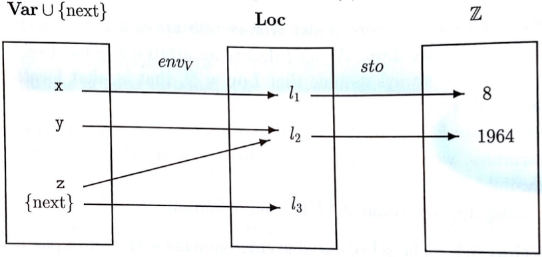
\includegraphics{resources/Images/stoloc.png}
    \caption{Environment-store model illustration \cite{stoloc}}
    \label{fig:Env}
\end{figure}

The following tables are the big step semantics of \lang{}.

\begin{table}[H]
\begin{adjustbox}{center}
\begin{tabular}{|c|c|}
\hline
\vspace {0.1pt} & \\
Num             &   \hbox{\Large \(env_V\, \vdash \langle n\: ,\ sto \rangle \rightarrow_a (v\: ,\ sto') \)\normalsize\(\quad \textbf{if}\ N\llbracket n \rrbracket = v  \)}  \vspace{0.1pt} \\ \hline 
\vspace {0.1pt} & \\  
Var             & \hbox{\Large \(env_V\, \vdash \langle x\: ,\ sto \rangle \rightarrow_a (v\: ,\ sto')\)\normalsize\( \quad \textbf{if} \: \begin{aligned}  env_V\ x=l \\ sto\ l = v \end{aligned} \)} \vspace {0.1pt} \\ \hline
\end{tabular}
\end{adjustbox}
    \caption{Num and var}
    \label{fig:declExp}
\end{table}

\begin{table}[H]
\begin{adjustbox}{center}
\begin{tabular}{|c|c|}
\hline
\vspace {0.1pt} & \\
Var-Decl      & \pbox{20cm}{ \huge \(\frac{env_C\, \vdash \langle D_V\: ,\ env_V']\rangle \rightarrow_{DV}\: (env'_V)}{env_C\, \vdash \langle dcl\ var\ x\ D_V\: ,\ env_V \rangle \rightarrow_{DV}\: env'_V} \)  \\ \\ \\ \normalsize \(  \textbf{where}\quad \: \begin{aligned} l=env_V\ next \\ env_V' = env_V[x \mapsto l][next \mapsto new\ l] \end{aligned} \)} \vspace {0.1pt} \\ \hline
\vspace {0.1pt} & \\
Empty-Var       & \hbox{\Large \(\langle \varepsilon\: ,\ env_V \rangle \rightarrow_{DV} env_V\)} \vspace {0.1pt} \\ \hline

\end{tabular}
\end{adjustbox}
    \caption{Declaration expressions}
    \label{fig:DeclarationExp}
\end{table}

\begin{table}[H]
\begin{adjustbox}{center}
\begin{tabular}{|c|c|}

\hline
\vspace {0.1pt} & \\
Relations 1     &   \pbox{20cm}{\Large \(env\, \vdash \langle a_1\: ,\ sto \rangle \rightarrow_a\: (v_1\: ,\ sto'')\) \\ \huge \(\frac{env\, \vdash \langle a_2\: ,\ sto'' \rangle \rightarrow_a\: (v_2\: ,\ sto')}{env\, \vdash \langle a_1\ op\ a_2\: ,\ sto' \rangle \rightarrow_b\: (\textit{tt}\: ,\ sto')}\)\normalsize\( \quad \begin{aligned} \textbf{if} \ v_1\ op\ v_2 \\ \textbf{where}\  op \in \{=, !=, >, <, >=, <= \}\end{aligned} \)}  \vspace{0.1pt} \\ \hline 
\vspace {0.1pt} & \\  
Relations 2     & \pbox{20cm}{\Large \(env\, \vdash \langle a_1\: ,\ sto \rangle \rightarrow_a\: (v_1\: ,\ sto'')\) \\ \huge \(\frac{env\, \vdash \langle a_2\: ,\ sto'' \rangle \rightarrow_a\: (v_2\: ,\ sto')}{env\, \vdash \langle a_1\ op\ a_2\: ,\ sto \rangle \rightarrow_b\: (\textit{ff}\: ,\ sto')}\)\normalsize\( \quad \begin{aligned} \textbf{if} \ \neg(v_1\ op\ v_2) \\ \textbf{where}\ op \in \{=, !=, >, <, >=, <= \}\end{aligned} \)} \vspace {0.1pt} \\ \hline
\vspace {0.1pt} & \\
Not 1           & \hbox{\huge\(\frac{env\, \vdash \langle b\: ,\ sto \rangle \rightarrow_b\: (\textit{tt}\: ,\ sto')}{env\, \vdash \langle not\ b\: ,\ sto \rangle \rightarrow_b\: (\textit{ff}\: ,\ sto')}\)} \vspace {0.1pt}\\ \hline
\vspace {0.1pt} & \\  
Not 2           & \hbox{\huge\(\frac{env\, \vdash \langle b\: ,\ sto \rangle \rightarrow_b\: (\textit{ff}\: ,\ sto')}{env\, \vdash \langle not\ b\: ,\ sto \rangle \rightarrow_b\: (\textit{tt}\: ,\ sto')}\) } \vspace {0.1pt}\\ \hline
\end{tabular}
\end{adjustbox}
    \caption{Boolean expressions}
    \label{fig:BooleanExp}
\end{table}

\begin{table}[H]
    \centering
    \begin{tabular}{|c|c|}

    \hline
    \vspace {0.1pt} & \\
And 1     & \pbox{20cm}{\Large \(env_V\, \vdash \langle b_1\: ,\ sto \rangle \rightarrow_b (\textit{tt}\: ,\ sto'')\) \\ \huge\(\frac{env_V\, \vdash \langle b_2\: ,\ sto'' \rangle \rightarrow_b\: (v\: ,\ sto')}{env_V\, \vdash \langle b_1\ and\ b_2\: ,\ sto \rangle \rightarrow_b (v\: ,\ sto')}\) } \vspace{0.1pt} \\ \hline 
    \vspace {0.1pt} & \\
And 2     & \hbox{\huge\(\frac{env_V\, \vdash \langle b_1\: ,\ sto \rangle \rightarrow_b (\textit{ff}\: ,\ sto')}{env_V\, \vdash \langle b_1\ and\ b_2\: ,\ sto \rangle \rightarrow_b (\textit{ff}\: ,\ sto')}\)} \vspace{0.1pt} \\ \hline 
    \vspace {0.1pt} & \\
Or 1     & \hbox{\huge\(\frac{env_V\, \vdash \langle b_1\: ,\ sto \rangle \rightarrow_b (\textit{tt}\: ,\ sto')}{env_V\, \vdash \langle b_1\ or\ b_2\: ,\ sto \rangle \rightarrow_b (\textit{tt}\: ,\ sto')}\)} \vspace{0.1pt} \\ \hline 
    \vspace {0.1pt} & \\
Or 2     & \pbox{20cm}{\Large \(env_V\, \vdash \langle b_1\: ,\ sto \rangle \rightarrow_b (\textit{ff}\: ,\ sto'')\) \\ \huge\(\frac{env_V\, \vdash \langle b_2\: ,\ sto'' \rangle \rightarrow_b\: (v\: ,\ sto')}{env_V\, \vdash \langle b_1\ or\ b_2\: ,\ sto \rangle \rightarrow_b\: (v\: ,\ sto')}\) }  \vspace{0.1pt} \\ \hline 
    \end{tabular}
    \caption{Gate expressions}
    \label{fig:GatesExp}
\end{table}

\begin{table}[H]
\begin{adjustbox}{center}
    \begin{tabular}{|c|c|}

    \hline
    \vspace {0.1pt} & \\
Parentheses & \hbox{\huge\(\frac{env_V\, \vdash \langle a\: ,\ sto \rangle \rightarrow_a\: (v\: ,\ sto')}{env_V\, \vdash \langle (a)\: ,\ sto \rangle \rightarrow_a\: (v\: ,\ sto')}\)} \vspace{0.1pt} \\ \hline 
    \vspace {0.1pt} & \\
    \(\begin{aligned}
\textrm{Addition} \\ \textrm{Subtraction} \\ \textrm{Multiplication}\end{aligned}\)  &   \pbox{20cm}{\Large\(env_V\, \vdash \langle a_1\: ,\ sto \rangle \rightarrow_a \: (v_1\: ,\ sto'')\) \\ \huge \(\frac{env_V\, \vdash \langle a_2\: ,\ sto'' \rangle \rightarrow_a\: (v_2\: ,\ sto')}{env_V\, \vdash \langle a_1\ op\ a_2\: ,\ sto \rangle \rightarrow_a \: (v\: ,\ sto')}\)\normalsize\( \quad \textbf{where} \quad op \in \{+,-,\cdot \} \)} \vspace{0.1pt} \\ \hline 
    \vspace {0.1pt} & \\
\(\begin{aligned}\textrm{Division} \\ \textrm{Modulo}\end{aligned}\)   & \pbox{20 cm}{\Large \(env_V\, \vdash \langle a_1\: ,\ sto \rangle \rightarrow_a (v_1\: ,\ sto'')\) \\ \huge \(\frac{env_V\, \vdash \langle a_2\: ,\ sto'' \rangle \rightarrow_a\: (v_2\: ,\ sto')}{env_V\, \vdash \langle a_1\ op\ a_2\: ,\ sto \rangle \rightarrow_a\: (v\: ,\ sto')}\)\normalsize\( \quad \textbf{where} \ \begin{aligned} op \in \{/,mod\} \\ v_2 \neq 0 \end{aligned} \)} \vspace{0.1pt} \\ \hline 
    \vspace {0.1pt} & \\
Unary   & \hbox{\huge\(\frac{env_V\, \vdash \langle a\: ,\ sto \rangle \rightarrow_a\: (v\: ,\ sto')}{env_V\, \vdash \langle -a\: ,\ sto \rangle \rightarrow_a\: (v\: ,\ sto')}\)\normalsize\( \quad \textbf{where} \quad v = -v\)} \vspace{0.1pt} \\ \hline 
    \end{tabular}
\end{adjustbox}
\caption{Arithmetic expressions}
\label{fig:ArithmeticExp}
\end{table}

\begin{table}[H]
\begin{adjustbox}{center}
\begin{tabular}{|c|c|}
\hline
\vspace {0.1pt} & \\
  if 1 &  \pbox{20cm}{\huge\(\frac{env_{VMC}\, \vdash \langle B_1\: ,\ sto'' \rangle \rightarrow (sto'\: ,\ Heap')}{ env_{VMC}\, \vdash \langle if\ b\ then\ B_1\ else\ B_2\ end\: ,\ sto\ \rangle \rightarrow sto'}\) \\ \normalsize\(\textbf{if} \quad env_V\, \vdash \langle b\: ,\ sto \rangle \rightarrow_b (\textit{tt}\: ,\ sto'')\)} \vspace{0.1pt} \\ \hline 
    \vspace {0.1pt} & \\
 if 2 &   \pbox{20cm}{\huge\(\frac{env_{VMC}\, \vdash \langle B_2\: ,\ sto'' \rangle \rightarrow (sto', Heap')}{ env_{VMC}\, \vdash \langle if\ b\ then\ B_1\ else\ B_2\ end\: ,\ sto\ \rangle \rightarrow sto'}\) \\ \normalsize\(\textbf{if} \quad env_V\, \vdash  \langle b\: ,\ sto \rangle \rightarrow_b (\textit{ff}\: ,\ sto'')\)} \vspace{0.1pt} \\ \hline 
    \vspace {0.1pt} & \\
  while 1 &  \pbox{20cm}{\Large \(env_{VMC}\, \vdash \langle B,\: sto'' \rangle \rightarrow (sto'''\: ,\ Heap'')\)\\
  \huge \(\frac{env_{VMC}\, \vdash \langle while\ b\ do\ B\ end\: ,\ sto'''\: ,\ Heap \rangle \rightarrow (sto'\: ,\ Heap)}{env_{VMC}\, \vdash \langle while\ b\ do\ B\ end\: ,\ sto \rangle \rightarrow (sto'\: ,\ Heap')} \) \\ \normalsize\(\textbf{if} \quad env_V\, \vdash \langle b\: ,\ sto \rangle \rightarrow_b (\textit{tt}\: ,\ sto'')\)} \vspace{0.1pt} \\ \hline 
\vspace {0.1pt} & \\
  while 2 &  \pbox{20cm}{\Large\(env_{VMC}\, \vdash \langle while\ b\ do\ B\ end\: ,\ sto\: ,\ Heap \rangle \rightarrow (sto'\: ,\ Heap)\) \\ \normalsize\(\textbf{if} \quad env_V\: ,\ env_C \, \vdash  \langle b\: ,\ sto \rangle \rightarrow_b (\textit{ff}\: ,\ sto')\)} \vspace{0.1pt} \\ \hline 
\vspace {0.1pt} & \\
  \(\begin{aligned} \textrm{for} \\ \textrm{upto 1} \end{aligned}\) &  \pbox{20cm}{\Large\(env_{VMC}\, \vdash \langle for\ x\ upto\ e\ do\ B\ end\: ,\ sto'\: ,\ Heap \rangle \rightarrow (sto'\: ,\ Heap) \) \\  \\ \normalsize \(\textbf{where}\ \begin{aligned} env_V\: ,\ env_C\, \vdash \langle x\: ,\ sto \rangle \rightarrow (v\: ,\ sto) \\ env_V\: ,\ env_C\, \vdash \langle e\: ,\ sto \rangle \rightarrow (v'\: ,\ sto')\\ v > v' \end{aligned}\) } \vspace{0.1pt} \\ \hline 
  \vspace {0.1pt} & \\
  \(\begin{aligned} \textrm{for} \\ \textrm{upto 2} \end{aligned}\) &  \pbox{20cm}{\Large \(env_{VMC}\, \vdash \langle B\: ,\ sto'' \rangle \rightarrow (sto'''\: ,\ Heap'')\) \\ \huge \(\frac{env_{VMC}\, \vdash \langle for\ x\ upto\ n\ do\ B\ end\: ,\ sto'''[l \mapsto v+1]\: ,\ Heap'' \rangle \rightarrow (sto'\: ,\ Heap')}{env_{VMC}\, \vdash \langle for\ x\ upto\ e\ do\ B\ end\: ,\ sto \rangle \rightarrow (sto'\: ,\ Heap')}\) \\ \\ \\ \normalsize\(\quad \textbf{where} \begin{aligned} env_V\: ,\ env_C\, \vdash \langle x\: ,\ sto \rangle \rightarrow (v\: ,\ sto) \\ env_V\: ,\ env_C\, \vdash \langle e\: ,\ sto \rangle \rightarrow (v'\: ,\ sto'') \\ n = N^{-1}[v'] \\ l=env_v\ x \\ v \leq v'  \end{aligned}\)} \vspace {0.1pt} \\ \hline
\end{tabular}
\end{adjustbox}
\caption{Control blocks}
    \label{fig:ControlBlock}
\end{table}

The 'for downto 1-2' are not displayed, as these are identical to 'for upto 1-2' with a few adjustments. The 'upto' operation is replaced with 'downto'. \(v\) has to, in 'downto 1', be less than \(v'\) instead of greater. In 'downto 2', \(v\) has to be greater than or equals \(v'\) instead of less than or equals. Lastly, \(l\) has to, in 'downto 2', map to \(v-1\) instead of \(v+1\). \\


For the sake of readability, \(env_V\: ,\ env_M\) are written as \(env_{VM}\) and \(env_V\: ,\ env_M\: ,\ env_C\) are written as \(env_{VMC}\). The for loop is split into four parts. Two for counting up and two for counting down, although the ones for counting down are, as mentioned above, not displayed. The 'for upto 1' is executed when the value of x is greater than the value of e. This is seen in the side conditions, where the value \(v\) of x, placed in \(sto\), has to be greater than the value \(v'\) of e, placed in \(sto''\), for it to be executed. Since the loop does not run, the storage does not change. 

The 'for upto 2' is executed when the value of x is smaller than the value of e. This is therefore the part that runs the statement in the for loop every time the before-mentioned side condition is true. The first precondition indicates that S is placed in sto''. The reason why this is not just \(sto\) is the fact that it is not necessarily the starting state. This state is executed and placed in \(sto'''\). The second precondition turns the value of e into a numeral with n, which is obtained as \(n = N^{-1}\llbracket v' \rrbracket \), and counts up the location defined by \(l = env_V\ x\) before placing it in \(sto'\).



%in the for upto 2 there is a bit more since this runs more then ones,  the first line \(\langle S,\ Sto''\rangle \rightarrow sto'''\) this say that it will run S, then in the next we count op the \(v\) of location l to \(v + 1\) and then ends, this can run if \(v \leq v'\) where x is stored in \(v\) and e is stored in the \(v'\), it also chance the value \(v'\) to the numerul n \(n=N^{-1}\llbracket v'\rrbracket\) and the location l is equal to the variable x in this enverememt.
\section{Scope Rules of \lang{}}
In \lang{}, the scope rules are fully static scope rules, as it has static scope rules for variables and static scope rules for functions. This means that both the variables and functions are bound when they are declared. 
\begin{comment}
\begin{table}[H]
    \begin{adjustbox}{center}
        \begin{tabular}{|c|c|}

\hline
\vspace {0.1pt}  &\\
PROC          &   \hbox{\huge \(\frac{env_V \vdash \langle D_P,\  env_P [p \mapsto (S,\  env_P)] \rangle \rightarrow_{DP} env'_P}{env_V \vdash \langle proc\ p\ is\ S;\ D_P,\ env_P \rangle \rightarrow_{DP} env'_P}\) } \vspace{0.1pt} \\ \hline 
\vspace {0.1pt} & \\  
PROC-EMPTY    & \hbox{\huge \(env_V \vdash \langle \varepsilon, env_P \rangle \rightarrow_{DP} env_P \)} \vspace {0.1pt} \\ \hline
\vspace {0.1pt} & \\ 
CALL-STAT-DYN & \hbox{\huge \(\frac{e'v[next \rightarrow e], e_p \vdash \langle S, \  st\rangle \rightarrow St'}{e_v , e_p \vdash \langle Call \  p, St \rangle \rightarrow St'} \ where \begin{aligned} e_p (p) = \langle S, e'_v \\ e = e_v (next) \end{aligned}\) } \vspace{0.1pt}  \\ \hline

        \end{tabular}
    \end{adjustbox}
    
    \caption{Caption}
    \label{fig:TrannyRulesProc}
\end{table}
\end{comment}
On the table \ref{fig:Func} the transition rules for function declarations are shown in the first two rows and the transition rule for function calls in the last row.


\begin{table}[H]
    \begin{adjustbox}{center}
        \begin{tabular}{|c|c|}
        \hline
\vspace {0.1pt} &\\
FUNC-Dcl        &   \hbox{\huge \(\frac{env_V\, \vdash \langle D_M\: ,\  env_M [f \mapsto (B\: ,\  env_M)] \rangle \rightarrow_{DM}\: env'_M}{env_V \vdash \langle func\ f(e_1\: ,\ ...\: ,\ e_n)\ begin\ B\ end\ D_M \ env_M \rangle \rightarrow_{DM}\: env'_M}\) } \vspace{0.1pt} \\ \hline 
\vspace {0.1pt} & \\  

Empty-FUNC-Dcl        &   \hbox{\Large \(env_V\, \vdash \langle \varepsilon\: ,\ env_F \rangle \rightarrow_{DF}\: env_F\) } \vspace{0.1pt} \\ \hline 
\vspace {0.1pt} & \\  

Func-Call  & \pbox{20cm}{\large \(env'_V\: ,\ env_M\, \vdash \langle B\: ,\ sto'' \rangle \rightarrow sto'\) \\ \huge \(\frac{env_M\, \vdash \langle PList\: ,\ sto\: ,\ env_V \rangle \rightarrow_{PList}(sto''\: ,\ env'_V)}{env\, \vdash \langle f(Plist)\: ,\ sto)\rightarrow sto'}\) \normalsize \\ \\ \(\textbf{Where} \quad PList \in \{x_1\: ,\ ...\: ,\ x_n\} \) } \vspace{0.1pt}  \\ \hline

        \end{tabular}
    \end{adjustbox}
    
    \caption{Functions call and declaration}
    \label{fig:Func}
\end{table}


\begin{table}[H]
    \begin{adjustbox}{center}
        \begin{tabular}{|c|c|}
        \hline
\vspace {0.1pt} &\\
EMPTY & \hbox{\Large \(env_V\: ,\ env_C\, \vdash \langle \varepsilon\: ,\ \varepsilon\: ,\ env_V\: ,\ sto \rangle \rightarrow (env_V\: ,\ sto)\)}\vspace{0.1pt} \\ \hline 
\vspace {0.1pt} & \\
ByRef & \pbox{20cm}{\huge \(\frac{\langle PList\: ,\ AList\: ,\ env''_V\: ,\ sto \rangle \rightarrow (env'_V\: ,\ sto')}{env_C\: ,\ env_C\, \vdash \langle y\ PList\: ,\ x\ AList\: ,\ env_V\: ,\ sto \rangle \rightarrow (env'_V\: ,\ sto')}\) \normalsize \\ \\ \(\textbf{Where} \begin{aligned} env_V[x\, \mapsto e] = env''_V \\ env_V(y) = e \end{aligned}\)} \vspace{0.1pt} \\ \hline 
\vspace {0.1pt} & \\
ByVal & \pbox{20cm}{\huge \(\frac{\langle PList\: ,\ AList\: ,\ env''_V\: ,\ sto'' \rangle \rightarrow (env'_V\: ,\ sto')}{env_V\: ,\ env_C\, \vdash \langle e\ PList\: ,\ x\ AList\: ,\ env_V\: ,\ sto \rangle \rightarrow (env'_V\: ,\ sto')}\) \normalsize \\ \\ \(\textbf{Where} \begin{aligned} env_V\, \vdash \langle e\: ,\ sto \rangle \rightarrow_e\: (v\: ,\ sto'') \\ env''_V = env_V[x\, \mapsto l][next\, \mapsto new\ l] \\ l = new(env_V\ next) \\ sto'' = sto[l \rightarrow v] \end{aligned} \)} \vspace{0.1pt} \\ \hline 
       
        \end{tabular}
    \end{adjustbox}
    
    \caption{PList Semantics}
    \label{fig:Plist}
\end{table}

In \lang{}, functions and a class constructor can take a set of defined parameters. These can both be by value and by reference. These is defined by PList. Their big-step semantics are defined in table \ref{fig:Plist}. The first rule, EMPTY, is called when the current parameter does not exist. Here, empty is returned. The Plist byRef starts with the \(env''_V\), as it is recursive, so there are possible information from earlier that needs to be taken into consideration. It saves the new information in the \(env'_V\) and \(sto'\), where the location of y is stored and passed on. The ByVal takes the value from the e that is in the \(env_V\) and stores the value from it in \(sto''\). Afterwards, it makes a new variable x that has a new location assigned to it, where it stores the value v.


\begin{table}[H]
    \begin{adjustbox}{center}
        \begin{tabular}{|c|c|}
        \hline
\vspace {0.1pt} &\\
Class-Dcl        &   \pbox{20cm}{\huge \(\frac{env_{VM}\, \vdash \langle P\: ,\ env''_C \rangle \rightarrow_{DC}\: env'_C}{env_{VM}\, \vdash \langle class\ c\ is\ c'\ begin\ D_V\ D_M\ end\ P\: ,\ env_C \rangle \rightarrow_{DC}\: env_C}\) \\ \\ \\ \normalsize \(\textbf{Where} \begin{aligned} env_C(c') = (env''_V\: ,\ env''_M) \\ env_C\, \vdash \langle D_V\: ,\ env''_V \rangle \rightarrow_{DV}\: env'_V \\ env'_V\, \vdash \langle D_M\: ,\ env''_M \rangle \rightarrow_{DM}\: env_M' \\ env''_C = env_C [c\, \mapsto(env_V'\: ,\ env_M')] \end{aligned} \)} \vspace{0.1pt} \\ \hline 
\vspace {0.1pt} & \\  

Class-instantiation &   \pbox{20cm}{\Large \(env''_V\: ,\ env_C\, \vdash \langle B\: ,\ sto''\: ,\ Heap \rangle \rightarrow (sto'\: ,\ Heap'')\) \\ \huge \(\frac{env_V\, ,\ env_C\, \vdash \langle PList\: ,\ AList\: ,\ env'_V\: ,\ sto \rangle \rightarrow (env''_V\: ,\ sto'')}{env_V\: ,\ env_C\, \vdash \langle set\ y\ to\ new\ c(PList)\: ,\ sto\: ,\ Heap \rangle \rightarrow (sto'\: ,\ Heap')}\) \\ \\ \\ \normalsize \(\textbf{Where} \begin{aligned} Heap' = Heap''[y\, \mapsto (env''_V\: ,\ sto\: ,\ Heap'')] \\ env_C(c) = (env'_V\: ,\ env_M) \\ env_M(OnConstruct) = (B\: ,\ AList\: ,\ env'_V) \end{aligned}\)} \vspace{0.1pt} \\ \hline
%Class-instantiation &   \pbox{20cm}{\Large \(env_C\, \vdash \langle D_V\: ,\ env_V\: ,\ sto \rangle \rightarrow (env''_V\: ,\ sto'')\) \\ \(env''_V\: ,\ env^1_C\, \vdash \langle D_M\: ,\ env^1_M \rangle \rightarrow env''_M\)\huge \\ \(\frac{env''_C\, \vdash \langle D_C\: ,\ envC[c\, \mapsto l]\: ,\ sto'''' \rangle \rightarrow \langle env'_V\: ,\ sto' \rangle}{env_C\, \vdash \langle set\ y\ to\ new\ c(Plist) \: ,\ env_C\: ,\ sto \rangle \rightarrow (env'_C\: ,\ sto')}\) \\ \\ \\ \normalsize \( \textbf{Where}\begin{aligned} env_C\ c = (B\: ,\ env_V\: ,\ env_M\: ,\ env_C) \\ l = sto'''\ next \\ sto'''' = sto'''[l \mapsto env''_V\: ,\ env''_M\: ,\ env''_C][next \mapsto new\ l] \end{aligned}\)} \vspace{0.1pt} \\ \hline 


    \end{tabular}
    \end{adjustbox}
    
    \caption{Caption}
    \label{fig:TrakhjnnyRulesProc}
\end{table}
    

When \lang{} returns a primitive value, the value is placed in a specific location, where it is retrievable after the function call. This location is called \textbf{retVar}, which is defined as: \(\textbf{retVar} = \textbf{Loc}\).

\begin{table}[H]
    \begin{adjustbox}{center}
        \begin{tabular}{|c|c|c|}
        \hline
\vspace {0.1pt} &\\
Assignment      &   \pbox{20cm}{\Large \(env_{VM}\, \vdash \langle set\ x\ to\ e\: ,\ sto \rangle \rightarrow sto'[l \mapsto v] \quad\)\\ \\ \( \textbf{where}\ \begin{aligned} env_{VM}\, \vdash \langle e\: ,\ sto \rangle \rightarrow \: (v\: ,\ sto') \\ l = env_V\ x \end{aligned} \) } \vspace{0.1pt} \\ \hline 
\vspace {0.1pt} & \\

Block       &   \pbox{20cm}{\Large \( \langle D_V\: ,\ env_V \rangle \rightarrow_{DV} env'_V \) \\ \huge \(\frac{env'_V\: ,\ env_M\, \vdash \langle S\: ,\ sto \rangle \rightarrow sto'}{env_{VM}\, \vdash \langle \{D_V\ S \}\: ,\ sto \rangle \rightarrow sto'} \) } \vspace{0.1pt} \\ \hline 
\vspace {0.1pt} & \\
Skip       &   \pbox{20cm}{\Large \( env_{VM}\, \vdash \langle skip\: ,\ sto \rangle \rightarrow sto \) } \vspace{0.1pt} \\ \hline 
\vspace {0.1pt} & \\

Composite       &   \pbox{20cm}{\Large \(env_{VM}\, \vdash \langle S_1\: ,\ sto \rangle \rightarrow sto''\) \\ \huge \(\frac{env_{VM}\, \vdash \langle S_2\: ,\ sto'' \rangle \rightarrow sto'}{env_{VM}\, \vdash \langle S_1\ S_2\: ,\ sto \rangle \rightarrow sto'}\) } \vspace{0.1pt} \\ \hline 
\vspace {0.1pt} & \\

Return Primitive          & \hbox{\huge \(\frac{env_{VM}\, \vdash \langle x\: ,\ retVar\: ,\ sto \rangle \rightarrow\: retVar'\: ,\ sto}{env_V\, \vdash \langle return\: x,\ env_V\: ,\ sto \rangle \rightarrow\: retVar'\: ,\ env_V\ sto}\) } \vspace{0.1pt}  \\ \hline
\vspace {0.1pt} & \\

Return Reference      & \hbox{\huge \(\frac{env_{VM}\, \vdash \langle y\: ,\ sto \rangle \rightarrow\: sto'}{env_V\, \vdash \langle return\: y,\ env_V\: ,\ sto \rangle \rightarrow\:  env_V'\ sto'}\) } \vspace{0.1pt}  \\ \hline

        \end{tabular}
    \end{adjustbox}
    \caption{Caption}
    \label{fig:hgf}
\end{table}

\begin{table}[H]
    \begin{adjustbox}{center}
        \begin{tabular}{|c|c|c|}
        \hline
\vspace {0.1pt} &\\
Program1      &   \pbox{20cm}{\Large \(env_V\, \vdash \langle D_V\: ,\ env_V\: ,\ sto \rangle \rightarrow (env''_V\: ,\ sto') \)\huge \\ \(\frac{env''_{VMC}\, \vdash \langle M_C\: ,\ env_C \rangle \rightarrow env'_C }{env_{VMC}\, \vdash \langle D_V\: ,\ M_C\: ,\ sto \rangle \rightarrow sto'} \) } \vspace{0.1pt} \\ \hline 
\vspace {0.1pt} & \\
Program2     &   \pbox{20cm}{\huge  \(\frac{env_{VMC}\, \vdash \langle D_C\: ,\ env_C \rangle \rightarrow env'_C }{env_{VMC}\, \vdash \langle D_C P\: ,\ sto \rangle \rightarrow sto'} \) } \vspace{0.1pt} \\ \hline 

        \end{tabular}
    \end{adjustbox}
    
    \caption{Program}
    \label{fig:progstuff}
\end{table}



This concludes the semantics chapter, where the abstract syntax was presented, the operational semantics were specified and where it was explained how the type rules and scope rules of \lang{} work. 
Now that all the semantics of \lang{} have been formally specified, a description of the implementation of \lang{} will follow.